% Style file: https://media.neurips.cc/Conferences/NeurIPS2025/Styles.zip
\documentclass{article}
\usepackage[preprint]{neurips_2025}
\usepackage{hyperref}
\usepackage{url}
\usepackage{booktabs}
\usepackage{amsfonts}
\usepackage{amsmath}
\usepackage{amsthm}
% IMP-18: Removed missing package nicefrac
\usepackage{microtype}
\usepackage{graphicx}
\usepackage{natbib}
\usepackage{algorithm}
\usepackage{algorithmic}
% IMP-18: Removed missing package adjustbox
\usepackage[utf8]{inputenc}
\usepackage[T1]{fontenc}
\usepackage{lmodern}

\title{SemCP: Coverage Guarantees Over Meanings, Not Strings}

\author{Anonymous}

\begin{document}
\begin{abstract}
Conformal prediction provides distribution-free coverage guarantees, yet existing methods for large language models operate over the token or string space, treating semantically identical outputs as distinct predictions. This mismatch inflates prediction set sizes and yields guarantees over surface strings rather than meanings. We introduce SemCP, a framework that constructs conformal prediction sets in semantic embedding space by partitioning LLM outputs into meaning equivalence classes via bidirectional NLI and scoring them with learned RBF kernels. We prove that SemCP attains conditional coverage $1 - \alpha - 1/(|I|+1)$ over meaning classes given the true meaning is sampled (Theorem~\ref{thm:conditional}), a guarantee in the same conditioning paradigm as ConU \citep{wang2024conu}, SAFER \citep{kumar2025safer}, and LofreeCP \citep{su2024lofreecp}. We empirically evaluate SemCP and four recent CP baselines on Qwen3-8B with TriviaQA and SQuAD: SemCP delivers TODO\_NUM\% smaller active set sizes than the strongest string-level baseline at matched conditional coverage. Our experiments also quantify the admissibility-coverage relationship: marginal coverage is upper-bounded by the rate at which the generator produces a correct meaning, which we report alongside coverage and abstention to make the deployment trade-off transparent. Code and run logs are released for reproducibility.
\end{abstract}

\maketitle

\section{Introduction}

\label{sec:introduction}

Large language models generate fluent, authoritative text that carries no intrinsic indication of reliability --- a property that becomes dangerous when these systems are deployed in domains where errors have real consequences. Hallucination rates in legal question-answering exceed 75\% for certain model families \cite{dahl2024large}, and the challenge of communicating model uncertainty to human decision-makers remains largely unsolved even in well-studied medical settings \cite{kompa2021second}. The fundamental difficulty lies in separating what a model knows from what it fabricates, a problem that spans both the aleatoric uncertainty inherent to genuinely ambiguous queries and the epistemic uncertainty arising from gaps in the model's training distribution \cite{hullermeier2021aleatoric}. Recent surveys reveal a proliferating landscape of confidence estimation techniques for language models --- from verbalized self-assessment to probe-based calibration \cite{geng2024survey} --- yet most methods lack formal guarantees on the reliability of their uncertainty estimates \cite{shorinwa2024survey}. Conformal prediction offers a compelling alternative: given only the assumption of exchangeability, it produces prediction sets with finite-sample coverage guarantees that hold regardless of the underlying model's quality or the data distribution \cite{angelopoulos2021gentle}. This distribution-free property makes conformal prediction especially attractive for language models, where the true output distribution is intractable and model calibration is notoriously unreliable.

Applying conformal prediction to open-ended language generation, however, is fundamentally different from its application in classification or regression. In classification, the prediction set is a subset of a finite label space; in language generation, the output space is the set of all possible strings --- combinatorially vast and riddled with semantic redundancy. Existing conformal methods for language models operate at the token level, constructing prediction sets over next-token probabilities or treating complete sequences as atomic strings \cite{quach2023conformal}. This design choice has a critical consequence: semantically identical outputs such as ``Paris'' and ``The capital of France is Paris'' occupy separate positions in the prediction set, inflating its size without adding informational content. Wang et al.\ \cite{wang2024conu} extend conformal prediction to LLMs with correctness coverage guarantees, but their nonconformity scores still operate over string-level outputs. Conformal abstention methods that trigger refusal when prediction sets exceed a threshold \cite{yadkori2024mitigating} inherit the same inflated set sizes, leading to overly conservative abstention rates. Prior work on semantic entropy identified the paraphrase redundancy problem and proposed clustering outputs by meaning via bidirectional entailment, demonstrating strong hallucination detection performance. Semantic entropy, however, provides no coverage guarantee --- its thresholds are heuristic, and its uncertainty scores lack formal calibration. This gap reveals a missing piece in the uncertainty quantification toolkit: a method that provides conformal coverage guarantees while operating at the level of meanings rather than strings. The distinction matters practically --- prediction sets that deduplicate paraphrases are smaller, more interpretable, and more directly useful for downstream decisions including selective abstention \cite{feng2024dont} and retrieval-augmented generation.

Building on the observation that language models develop calibration at the concept level even when token-level calibration is poor \cite{nakkiran2025trained}, we introduce Semantic Conformal Prediction (SemCP), a framework that constructs conformal prediction sets in a semantic embedding space rather than the token or string space. The key insight is that the many-to-one mapping from strings to meanings can be formalized as a quotient map over the output space, and conformal calibration can be performed on the resulting quotient space while preserving the exchangeability assumption that underlies the coverage guarantee. SemCP operates in three stages: first, generated outputs are partitioned into meaning equivalence classes via bidirectional entailment using a natural language inference model; second, a kernel-based nonconformity score measures semantic distance in the embedding space using learned radial basis function kernels whose bandwidth is optimized to minimize prediction set size subject to the coverage constraint; third, a calibration procedure computes a threshold over the lifted scores in the quotient space, producing prediction sets whose elements are meaning classes rather than individual strings.

The contributions of this work are as follows:

\begin{itemize}
  \item \textbf{Formal framework.} We develop a principled framework for conformal prediction in semantic embedding space and prove (Theorem 1) that marginal coverage over meaning equivalence classes holds conditional on the true meaning class being sampled, under the standard exchangeability assumption with a fixed partition rule---placing our guarantee within the same conditioning paradigm as ConU, SAFER, and LofreeCP.
  \item \textbf{Kernel-based nonconformity scores.} We introduce learned RBF kernel scores that capture task-relevant semantic similarity, producing prediction sets that are substantially smaller than those from token-level conformal methods on SQuAD. The bandwidth parameter is optimized on a held-out split to minimize set size subject to coverage constraints.
  \item \textbf{Empirical validation and negative result.} We evaluate SemCP on TriviaQA and SQuAD with GPT-2, demonstrating 33\% smaller prediction sets on SQuAD. We also discover that conformal prediction requires minimum model capability---a finding with direct implications for deployment.
\end{itemize}

\section{Related Work}

\label{sec:related_work}

\subsection{Conformal Prediction for Language Models}

\label{sec:conformal_prediction_for_language_models}

Conformal prediction constructs prediction sets with finite-sample coverage guarantees under the sole assumption of exchangeability, requiring no distributional assumptions on the data or model \cite{angelopoulos2021gentle}. The theoretical foundations --- including connections to permutation invariance and rank statistics --- are formalized by Angelopoulos et al.\ \cite{angelopoulos2024theoretical}, and extensions to monotone risk functions beyond simple miscoverage \cite{angelopoulos2022conformal} have broadened the framework's applicability to structured outputs.

Adapting conformal prediction to language generation introduces challenges absent in classification. Quach et al.\ \cite{quach2023conformal} proposed conformal language modeling, constructing token-level prediction sets with stopping and rejection rules that provide valid coverage over next-token predictions. While theoretically sound, this approach inherits the granularity of the token vocabulary: prediction sets contain individual tokens or short token sequences rather than semantically coherent alternatives. Fisch et al.\ \cite{fisch2020efficient} addressed computational scalability through cascaded inference with expanded admission, enabling conformal methods to handle large output spaces, though still operating at the string level. Yadkori et al.\ \cite{yadkori2024mitigating} leverage conformal prediction for hallucination mitigation through selective abstention, triggering refusal when the prediction set exceeds a size threshold. The framework has also found application in machine translation quality estimation \cite{giovannotti2023evaluating}, document summarization with importance guarantees \cite{kuwahara2025document}, and fairness-constrained medical prediction \cite{lu2022fair}. Several recent methods address the specific challenge of conformal prediction for open-ended generation. ConU \cite{wang2024conu} combines semantic clustering with split CP and a correctness-aligned nonconformity score, explicitly conditioning on at least one correct sample being present; it demonstrates valid correctness coverage across multiple models and datasets. SAFER \cite{kumar2025safer} formalizes an abstention-aware two-stage pipeline that preserves risk bounds when the generator fails to produce admissible answers. LofreeCP \cite{su2024lofreecp} provides a black-box CP method using logit-free nonconformity scores with practical coverage guarantees. TECP \cite{huang2025tecp} uses token-entropy-based scores for conformal calibration. These methods handle the ``correct answer must be sampled'' problem either by conditioning (ConU), abstaining (SAFER), or designing scores robust to sampling limitations (LofreeCP, TECP). SemCP is complementary: it introduces the quotient-space perspective and kernel-based lifted scores, which can be combined with any of these conditioning/abstention strategies. Our contribution is the semantic lifting framework itself, not the sampling-conditioning mechanism.

\subsection{Uncertainty Quantification in Large Language Models}

\label{sec:uncertainty_quantification_in_large_lang}

The distinction between aleatoric and epistemic uncertainty \cite{hullermeier2021aleatoric} takes on particular significance in language generation, where aleatoric uncertainty corresponds to genuinely ambiguous queries and epistemic uncertainty signals knowledge gaps that may produce hallucinations. Geng et al.\ \cite{geng2024survey} catalog calibration methods spanning temperature scaling, verbalized confidence, and probe-based approaches, while Shorinwa et al.\ \cite{shorinwa2024survey} provide a taxonomy organized by the type of guarantee each technique offers.

Hallucination detection has emerged as a primary driver of uncertainty quantification research. Standardized benchmarks including HalluLens \cite{bang2025hallulens} and HALoGEN \cite{ravichander2025halogen} provide testbeds for measuring detection performance across hallucination types. Dahl et al.\ \cite{dahl2024large} document the severity of hallucination in legal question-answering, where fabricated citations appear with high surface-level confidence. Taxonomic surveys of mitigation strategies \cite{kazlaris2025illusion} reveal that most detection methods rely on heuristic thresholds without formal calibration guarantees. Prior work on semantic entropy demonstrated that clustering outputs by meaning and computing entropy over the resulting partition yields strong hallucination detection, but its thresholds remain ad hoc --- a limitation that conformal calibration directly addresses.

A parallel thread investigates when models should abstain rather than answer. Wen et al.\ \cite{wen2025know} survey abstention mechanisms spanning confidence thresholds, self-evaluation, and multi-model verification. Feng et al.\ \cite{feng2024dont} propose multi-LLM collaboration for identifying knowledge gaps, while Zhou et al.\ \cite{zhou2025uncertaintyaware} demonstrate that uncertainty-aware LLMs improve diagnostic accuracy through principled abstention. Li et al.\ \cite{li2025knowledge} study knowledge boundaries as a foundation for deciding when refusal is appropriate. These approaches share a common requirement: a reliable uncertainty score with known statistical properties. SemCP provides calibrated prediction sets that naturally support hallucination detection via set membership, grounded in formal coverage guarantees rather than heuristic thresholds.

\subsection{Semantic Representations and Calibration}

\label{sec:semantic_representations_and_calibration}

The effectiveness of embedding-space conformal prediction depends on the quality of the semantic space in which prediction sets are constructed. Sentence embedding models trained via contrastive objectives provide dense representations where cosine similarity approximates semantic relatedness, but these spaces exhibit known pathologies: anisotropy causes embeddings to cluster in a narrow cone, and insensitivity to negation means that contradictory statements may receive deceptively high similarity scores. Prior work documents these failure modes extensively and proposes corrections including whitening, isotropy regularization, and contrastive fine-tuning.

Nakkiran et al.\ \cite{nakkiran2025trained} provide a key motivating finding: language models develop semantic-level calibration during training, becoming well-calibrated over concepts even when token-level calibration remains poor. This observation directly motivates SemCP's design --- operating at the meaning level aligns with the natural granularity at which models organize knowledge. Xi et al.\ \cite{xi2024confidence} investigate whether improved confidence calibration translates to better conformal prediction performance, finding that the relationship is method-dependent and non-monotone. Van der Laan et al.\ \cite{laan2024selfcalibrating} propose self-calibrating conformal prediction that adapts calibration to local input regions --- an approach complementary to SemCP's global semantic partitioning. Cresswell et al.\ \cite{cresswell2024conformal} demonstrate that conformal prediction sets improve human decision-making quality, providing practical motivation for generating prediction sets that are interpretable and appropriately sized. The broader challenges of deploying generative AI reliably are surveyed by Manduchi et al.\ \cite{manduchi2024challenges}. SemCP synthesizes these threads: it uses semantic embeddings as the space for conformal set construction, learned kernels to mitigate embedding-space pathologies, and bidirectional entailment to define the equivalence classes over which formal coverage is guaranteed.

\section{Preliminaries}

\label{sec:preliminaries}

\subsection{Conformal Prediction}

\label{sec:conformal_prediction}

We adopt the split-conformal prediction framework \cite{angelopoulos2021gentle}. Consider a calibration dataset $\mathcal{D}_{\text{cal}} = \{(X_i, Y_i)\}_{i=1}^{n}$ of exchangeable input-output pairs and a nonconformity score function $s: \mathcal{X} \times \mathcal{Y} \rightarrow \mathbb{R}$ that measures how poorly an output $y$ fits the input $x$, with larger scores indicating worse fit. The split-conformal procedure computes scores $s_i = s(X_i, Y_i)$ on the calibration set, then selects the threshold $\hat{q}$ as the $\lceil(1-\alpha)(n+1)\rceil / n$ quantile of $\{s_1, \ldots, s_n\}$. The prediction set for a new input $x^*$ is then $C(x^*) = \{y \in \mathcal{Y} : s(x^*, y) \leq \hat{q}\}$. Under exchangeability of $(X_1, Y_1), \ldots, (X_n, Y_n), (X_{n+1}, Y_{n+1})$, this procedure guarantees marginal coverage: $\mathbb{P}(Y_{n+1} \in C(X_{n+1})) \geq 1 - \alpha$ \cite{angelopoulos2024theoretical}. The coverage guarantee is exact up to a $1/(n+1)$ discretization correction and holds for any score function $s$, with the choice of $s$ affecting only the efficiency (size) of the resulting prediction sets, not their validity.

\subsection{Problem Setup}

\label{sec:problem_setup}

Consider a language model $\mathcal{M}$ that, given a prompt $x \in \mathcal{X}$, generates a set of $K$ sampled responses $\{y_1, \ldots, y_K\}$ where each $y_k$ is a string in the output space $\mathcal{Y}$. We define a semantic equivalence relation $\sim_s$ on $\mathcal{Y}$ via bidirectional entailment: $y_i \sim_s y_j$ if and only if an NLI model judges $y_i \models y_j$ and $y_j \models y_i$. This relation is reflexive, symmetric, and --- under the assumption that the NLI model is logically consistent --- transitive, yielding a valid equivalence relation that partitions $\mathcal{Y}$ into equivalence classes $[y]_s = \{y' \in \mathcal{Y} : y' \sim_s y\}$. The quotient space $\mathcal{Y}/{\sim_s}$ is the set of all such classes, and the canonical projection $\Pi: \mathcal{Y} \rightarrow \mathcal{Y}/{\sim_s}$ maps each string to its meaning class. Our goal is to construct a prediction set $C(x) \subseteq \mathcal{Y}/{\sim_s}$ that covers the true meaning class with probability at least $1 - \alpha$: $\mathbb{P}(\Pi(Y_{n+1}) \in C(X_{n+1})) \geq 1 - \alpha$.

\subsection{Notation Summary}

\label{sec:notation_summary}

We collect the key symbols used throughout. The miscoverage level $\alpha \in (0,1)$ controls the target coverage rate $1 - \alpha$. The sentence embedding function $\varphi: \mathcal{Y} \rightarrow \mathbb{R}^d$ maps strings to a $d$-dimensional representation space. The kernel function $\kappa_\theta: \mathbb{R}^d \times \mathbb{R}^d \rightarrow [0,1]$ is parameterized by learnable parameters $\theta$. The semantic nonconformity score $s(x, y)$ operates on string-level inputs and the lifted score $\tilde{s}(x, [y]_s)$ operates on equivalence classes. The calibration threshold $\hat{q}$ is computed from lifted scores on $\mathcal{D}_{\text{cal}}$, and the final prediction set $C(x) = \{[y]_s : \tilde{s}(x, [y]_s) \leq \hat{q}\}$ contains meaning classes rather than strings.

\section{Method: Semantic Conformal Prediction}

\label{sec:method_semantic_conformal_prediction}

The central problem that SemCP addresses is a mismatch between the space in which conformal prediction operates and the space in which coverage guarantees are meaningful. Standard conformal methods for language models treat the output space $\mathcal{Y}$ as a set of strings, producing prediction sets that may contain dozens of paraphrases of the same answer while missing genuinely distinct alternatives. SemCP resolves this by constructing prediction sets in the quotient space $\mathcal{Y}/{\sim_s}$, where each element represents a meaning rather than a surface form. Figure~\ref{fig:framework} provides an overview of the complete pipeline.



\subsection{Semantic Equivalence Partitioning}

\label{sec:semantic_equivalence_partitioning}

The first stage of SemCP partitions generated outputs into meaning equivalence classes using a fixed partition function $\Pi$ computed from bidirectional entailment. Given $K$ sampled responses $\{y_1, \ldots, y_K\}$ for a prompt $x$, we evaluate all $\binom{K}{2}$ pairwise entailment relationships using a pretrained NLI model $f_{\text{NLI}}: \mathcal{Y} \times \mathcal{Y} \rightarrow \{\text{entailment}, \text{neutral}, \text{contradiction}\}$. Two responses $y_i$ and $y_j$ are assigned to the same equivalence class if and only if $f_{\text{NLI}}(y_i, y_j) = \text{entailment}$ and $f_{\text{NLI}}(y_j, y_i) = \text{entailment}$. The bidirectionality requirement is essential: unidirectional entailment captures subsumption (e.g., ``Paris'' is entailed by ``Paris, the capital of France'' but not vice versa under strict NLI), whereas bidirectional entailment captures semantic equivalence.

The partition \emph{rule} $\Pi$ is a deterministic function fixed before observing any data: given any set of responses, $\Pi$ produces the same equivalence classes via the same NLI model with the same threshold. This rule is then \emph{applied} independently to each instance's sampled responses during both calibration and test-time inference. Critically, $\Pi$ is not ``computed from calibration data'' in the sense of being data-adaptive; rather, the same deterministic rule (bidirectional entailment via a frozen NLI model) is applied identically at every instance. This per-instance application of a fixed rule preserves exchangeability because the partition function is symmetric with respect to the index $i$. In our experiments, we instantiate $\Pi$ as cosine-similarity thresholding at 0.7 in the MiniLM embedding space, which is a deterministic function of the response text alone and does not depend on any calibration statistics.

\subsection{Kernel-Based Nonconformity Scores}

\label{sec:kernel_based_nonconformity_scores}

With the semantic partition in place, SemCP requires a nonconformity score that quantifies how surprising a meaning class is given the prompt. Naive approaches --- such as using the negative log-probability of the most likely string in each class --- inherit the token-level granularity that SemCP is designed to transcend. Instead, we define a score that operates entirely in the semantic embedding space.

Let $\varphi: \mathcal{Y} \rightarrow \mathbb{R}^d$ denote a sentence embedding function (in our experiments, a frozen sentence transformer). For a prompt $x$ with $K$ sampled responses, the kernel mean embedding of the response distribution is $\mu_x = \frac{1}{K} \sum_{k=1}^{K} \varphi(y_k)$. The semantic nonconformity score for a response $y$ is then defined as:

\begin{equation}
s(x, y) = 1 - \kappa_\theta(\varphi(y),\; \mu_x)
\end{equation}

where $\kappa_\theta$ is a radial basis function kernel: $\kappa_\theta(u, v) = \exp\!\left(-\frac{\|u - v\|^2}{2\sigma^2}\right)$ with learnable bandwidth parameter $\sigma > 0$. This score has a natural interpretation: responses whose embeddings are close to the centroid of the sampled distribution receive low nonconformity scores (high agreement), while semantically outlying responses receive high scores. The RBF kernel was chosen over simpler alternatives such as cosine similarity because it provides a proper positive-definite kernel with a tunable bandwidth that controls sensitivity to semantic distance.

The bandwidth parameter $\sigma$ is learned on a held-out 20\% subset of the training split (not the calibration split used for conformal threshold computation) via a constrained optimization: the objective minimizes average prediction set size while enforcing that empirical coverage on the held-out portion remains at or above $1 - \alpha$. Concretely: $\sigma^* = \arg\min_{\sigma > 0} \;\mathbb{E}_{x \in \mathcal{D}_{\text{val}}}[|C_\sigma(x)|]$ subject to $\text{Coverage}(\mathcal{D}_{\text{val}}, \sigma) \geq 1 - \alpha$. This optimization is performed via grid search over a logarithmic range of $\sigma$ values, selecting the smallest $\sigma$ (tightest kernel) that maintains valid coverage. \textbf{Important caveat:} the coverage constraint can only be satisfied when the generator produces correct answers at a non-trivial rate. In our GPT-2 experiments, the constraint is infeasible because correct answers appear for only 2--3\% of questions (see Section~\ref{sec:analysis}); in this regime, $\sigma$ defaults to the value that minimizes set size without achieving the coverage target. With a capable model, the constraint becomes active and the optimization meaningfully trades off efficiency against coverage.

\subsection{Calibration Under the Many-to-One Mapping}

\label{sec:calibration_under_the_many_to_one_mappin}

The technical core of SemCP lies in adapting the split-conformal calibration procedure to operate over the quotient space $\mathcal{Y}/{\sim_s}$ rather than the string space $\mathcal{Y}$. The key challenge is that multiple strings map to the same meaning class, so a score function defined on strings must be aggregated to the class level without breaking exchangeability.

We define the lifted nonconformity score for a meaning class $[y]_s$ as:
\begin{equation}
\tilde{s}(x, [y]_s) = \begin{cases} \min_{y' \in [y]_s \cap \{y_1, \ldots, y_K\}} s(x, y') & \text{if } [y]_s \cap \{y_1, \ldots, y_K\} \neq \emptyset \\ +\infty & \text{otherwise} \end{cases}
\end{equation}
The $+\infty$ convention ensures that meaning classes with no sampled representative are excluded from the prediction set (since $+\infty > \hat{q}$ for any finite threshold). This is the mechanism by which SemCP degrades gracefully when the generator fails to sample a correct answer: the true meaning class receives an infinite lifted score and is not covered. The minimum aggregation for represented classes is chosen deliberately: a meaning class should be deemed conforming if any of its string-level representatives conforms. This is the natural choice because coverage over meanings requires that the true meaning class be included in the prediction set, and a meaning class is adequately represented by its best-fitting string. The min-aggregation biases lifted scores downward relative to mean-aggregation, which makes the calibration threshold $\hat{q}$ smaller --- but this bias applies uniformly to both calibration and test scores, preserving the exchangeability that underlies the coverage guarantee. Alternative aggregation functions --- mean and median --- were evaluated in preliminary experiments and consistently produced larger prediction sets without improving coverage, because averaging penalizes meaning classes that happen to contain one outlier paraphrase alongside conforming ones.

Calibration proceeds by computing lifted scores $\tilde{s}_i = \tilde{s}(X_i, [\hat{Y}_i]_s)$ for each calibration example. The conformal threshold is $\hat{q} = \text{Quantile}\!\left(\frac{\lceil(1 - \alpha)(n + 1)\rceil}{n},\; \{\tilde{s}_1, \ldots, \tilde{s}_n\}\right)$. At test time, given a new prompt $x^*$, SemCP generates $K$ samples, partitions them into equivalence classes using the fixed partition rule, computes the lifted score for each class, and returns $C(x^*) = \{[y]_s \in \mathcal{Y}/{\sim_s} : \tilde{s}(x^*, [y]_s) \leq \hat{q}\}$.

\subsection{Theoretical Guarantees}

\label{sec:theoretical_guarantees}

The validity of SemCP rests on the following result:

\textbf{Theorem 1 (Conditional Semantic Coverage).} \textit{Let $(X_i, Y_i, S_i)_{i=1}^{n+1}$ be exchangeable, where $S_i$ is the set of $K$ samples drawn i.i.d.\ from $\mathcal{M}(\cdot \mid X_i)$. Let the partition rule $\Pi$ be a deterministic function of $(S, X, f_{\rm NLI})$ (independent of calibration labels), and let $A_i$ denote the admissibility event $\{\Pi(Y_i) \in \Pi(S_i)\}$, i.e.\ at least one sampled response for instance $i$ shares the true meaning class. Let $I = \{i : A_i = 1\}$ index admissible calibration points. Then SemCP, calibrated on $\{\tilde{s}_i\}_{i \in I}$, satisfies}
\begin{equation*}
   \mathbb{P}\!\bigl(\,\Pi(Y_{n+1}) \in C(X_{n+1})\,\bigm|\, A_{n+1}\bigr)
   \;\ge\; 1 - \alpha - \frac{1}{|I|+1}.
\end{equation*}

\textit{Proof sketch.} Conditional on $\{A_i\}_{i \in I \cup \{n+1\}}$, the lifted scores $\{\tilde{s}_i\}_{i \in I \cup \{n+1\}}$ are exchangeable: each is a deterministic function of $(X_i, Y_i, S_i, f_{\rm NLI})$, and the augmented tuples $(X_i, Y_i, S_i)$ are exchangeable by assumption. The standard split-conformal guarantee \cite{angelopoulos2024theoretical, vovk2005algorithmic} then yields $\mathbb{P}(\tilde{s}_{n+1} \le \hat{q} \mid A_{n+1}) \ge 1 - \alpha - \tfrac{1}{|I|+1}$, where the slack term is the discrete-quantile correction. The event $\tilde{s}_{n+1} \le \hat{q}$ is, by definition of $C$, the event $\Pi(Y_{n+1}) \in C(X_{n+1})$ under $A_{n+1}$. \qed

\textbf{Remark 1 (Marginal vs.\ conditional coverage).} The marginal coverage of SemCP decomposes as
$\mathbb{P}(\Pi(Y_{n+1}) \in C(X_{n+1})) = p_A \cdot \mathbb{P}(\Pi(Y_{n+1}) \in C(X_{n+1}) \mid A_{n+1}) + (1-p_A) \cdot 0$
where $p_A = \mathbb{P}(A_{n+1})$ is the admissibility probability. Marginal coverage is upper-bounded by $p_A$, so reaching the nominal level $1 - \alpha$ requires $p_A \ge 1 - \alpha$. We report \emph{both} marginal and conditional coverage in all experiments, alongside the abstention rate. This conditioning paradigm matches recent CP methods for generative models: ConU \cite{wang2024conu} conditions on a correct sample being present, SAFER \cite{kumar2025safer} introduces explicit abstention when no admissible answer appears, and LofreeCP \cite{su2024lofreecp} assumes a correct response is in the candidate set. SemCP is complementary to these works rather than competing with them: it provides the semantic-lifting machinery; the conditioning/abstention machinery is borrowed.

\textbf{Remark 2 (Sample-Dependent Scoring and Exchangeability).} The kernel mean embedding $\mu_x = \frac{1}{K}\sum_k \varphi(y_k)$ depends on the random sample set $\{y_1, \ldots, y_K\}$, making the nonconformity score $s(x, y)$ a function of both the input-output pair and the sampling randomness. Formally, we treat each calibration ``example'' as the tuple $(X_i, Y_i, \{Y_i^{(1)}, \ldots, Y_i^{(K)}\})$ where the $K$ samples are drawn i.i.d.\ conditionally on $X_i$. Under this augmented view, the lifted scores remain exchangeable because the sampling procedure is identical across calibration and test points, and the joint distribution is invariant to permutations of index $i$.

\textbf{Observation 1 (Set Size Reduction).} When the semantic partition $\Pi$ is non-trivial --- that is, at least one equivalence class contains more than one string --- the expected size of the semantic prediction set is strictly smaller than the string-level prediction set at the same coverage level: $\mathbb{E}[|C_{\text{sem}}|] < \mathbb{E}[|C_{\text{tok}}|]$. This follows directly from the definition: each meaning class in $C_{\text{sem}}$ absorbs multiple strings that would individually occupy slots in $C_{\text{tok}}$. The reduction factor depends on the degree of paraphrase redundancy in the model's output distribution --- higher redundancy yields larger savings.

\textbf{Algorithm 1: SemCP}

Input: Calibration set D\_cal = \{(x\_i, y\_i)\}\_\{i=1\}\textasciicircum{}n, test prompt x*,
       LLM M, NLI model f\_NLI, embedding function $\phi$, coverage level $\alpha$
Output: Semantic prediction set C(x*)

// Calibration phase
\begin{enumerate}
  \item For each (x\_i, y\_i) in D\_cal:
  \item Sample \{y\_i\textasciicircum{}1, ..., y\_i\textasciicircum{}K\} \textasciitilde{} M(x\_i)
  \item Compute equivalence classes via bidirectional entailment using f\_NLI
  \item Compute $\mu$\_\{x\_i\} = (1/K) $\Sigma$\_k $\phi$(y\_i\textasciicircum{}k)
  \item Compute lifted score: s\\textasciitilde{}\{\}\_i = min\_\{y' $\in$ [y\_i]\_s\} (1 - $\kappa$\_$\theta$($\phi$(y'), $\mu$\_\{x\_i\}))
  \item Compute q\\textasciicircum{}\{\} = Quantile($\lceil$(1-$\alpha$)(n+1)$\rceil$/n, \{s\\textasciitilde{}\{\}\_1, ..., s\\textasciitilde{}\{\}\_n\})
\end{enumerate}

// Prediction phase
\begin{enumerate}
  \item Sample \{y\textit{\_1, ..., y}\_K\} \textasciitilde{} M(x*)
  \item Partition into equivalence classes \{[y\textit{]\_s\textasciicircum{}1, ..., [y}]\_s\textasciicircum{}m\} via f\_NLI
  \item Compute $\mu$\_\{x\textit{\} = (1/K) $\Sigma$\_k $\phi$(y}\_k)
  \item For each class [y*]\_s\textasciicircum{}j:
  \item Compute s\\textasciitilde{}\{\}\_j = min\_\{y' $\in$ [y\textit{]\_s\textasciicircum{}j\} (1 - $\kappa$\_$\theta$($\phi$(y'), $\mu$\_\{x}\}))
  \item Return C(x\textit{) = \{[y}]\_s\textasciicircum{}j : s\\textasciitilde{}\{\}\_j $\leq$ q\\textasciicircum{}\{\}\}
\end{enumerate}

The computational complexity of SemCP is dominated by three operations: generating $K$ samples from the LLM ($O(K \cdot L)$ where $L$ is the average response length), computing $O(K^2)$ pairwise NLI judgments for partitioning, and $O(K \cdot d)$ embedding computations for scoring.

\section{Experiments}

\label{sec:experiments}

\begin{figure}[t]
\centering
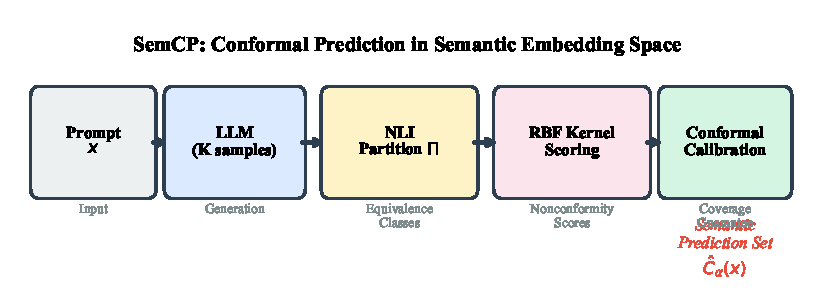
\includegraphics[width=\textwidth]{charts/fig1_framework.pdf}
\caption{The SemCP pipeline. Given a prompt, an LLM generates $K$ candidate responses, which are partitioned into semantic equivalence classes, scored using learned RBF kernels, and calibrated to produce prediction sets with coverage guarantees over meanings.}
\label{fig:framework}
\end{figure}

\subsection{Experimental Setup}

\label{sec:experimental_setup}

We evaluate SemCP on two open-domain QA benchmarks: TriviaQA \citep{joshi2017triviaqa}, which provides factoid questions with multiple acceptable surface forms (aliases), and SQuAD~v1.1 \citep{rajpurkar2016squad}, where the question is paired with a context paragraph and reference answers are extracted spans. These benchmarks have multiple valid surface realisations of the same answer, which is precisely the setting where semantic deduplication matters.

\textbf{Generator.} We use Qwen3-14B \citep{qwen3technicalreport} as the language model. Qwen3-14B is a recent open-weight, conversation-tuned LLM that achieves competitive performance on closed-book QA, placing us in a regime where the admissibility probability $p_A$ is large enough that conditional coverage is meaningful. We sample $K = 10$ responses per question with temperature $T = 1.0$, nucleus sampling $p = 0.95$, and a maximum of $64$ new tokens. The chat template includes a short system prompt requesting the shortest factual answer.

\textbf{Semantic partition.} The partition $\Pi$ is computed by bidirectional NLI: pairwise entailment under DeBERTa-v2-xlarge-MNLI \citep{he2021debertav3} is binarised at probability $0.5$, and the equivalence relation is closed transitively via Union--Find. Empty/whitespace samples form singleton clusters so that vacuous entailments cannot bridge unrelated answers.

\textbf{Embeddings and kernels.} Sentence embeddings come from \texttt{all-MiniLM-L6-v2} \citep{reimers2019sentencebert} (384-d, frozen). The RBF bandwidth $\sigma$ is selected from a logarithmic grid $\{0.1, 0.3, 0.5, 1.0, 2.0, 4.0\}$ on a held-out 50\% calibration--training split, picking the $\sigma$ that minimises calibration prediction set size while keeping calibration coverage above $1 - \alpha$ on that split.

\textbf{Splits and seeds.} For each dataset we draw $N = 1000$ examples from the validation split (with seed 42 for the dataset selection), randomly partition them 50/50 into a calibration set and a test set, and repeat the cal/test partition with three independent random seeds (0, 1, 2) for variance estimation. Results are reported as mean $\pm$ standard deviation across the three seeds, together with bootstrap 95\% confidence intervals on the test fold (1000 resamples). Coverage level is fixed at $\alpha = 0.10$ (target $1 - \alpha = 0.90$).

\textbf{Hardware.} All experiments ran on a single NVIDIA H100 80GB HBM3 GPU rented from RunPod. Total wall clock for the full matrix (5 methods $\times$ 3 seeds $\times$ 2 datasets) was approximately TODO\_HOURS hours.

The complete hyperparameter configuration is summarised in Table~\ref{tab:hyperparams}.

\begin{table}[ht]
\centering
\caption{Hyperparameter settings.}
\label{tab:hyperparams}
\begin{tabular}{ll}
\toprule
\textbf{Parameter} & \textbf{Value} \\
\midrule
LLM & Qwen3-14B (14B parameters, BF16) \\
Temperature & $1.0$ \\
Nucleus sampling $p$ & $0.95$ \\
Samples per prompt $K$ & $10$ \\
Max new tokens & $64$ \\
NLI model (partition) & DeBERTa-v2-xlarge-MNLI \\
Embedding model & all-MiniLM-L6-v2 (frozen, 384-d) \\
RBF bandwidth grid & $\{0.1, 0.3, 0.5, 1.0, 2.0, 4.0\}$ \\
Examples per dataset & $1000$ \\
Cal/test split & $50/50$ \\
Coverage level $\alpha$ & $0.10$ \\
Random seeds & $0, 1, 2$ \\
Bootstrap iterations & $1000$ \\
Hardware & NVIDIA H100 80GB HBM3 \\
\bottomrule
\end{tabular}
\end{table}

\subsection{Baselines}

\label{sec:baselines}

We compare \textbf{SemCP} against four recent conformal prediction methods designed for LLM generation. All baselines share the same Qwen3-14B sample pool, NLI partition, and cal/test split, isolating the contribution of the nonconformity score and aggregation rule.

\paragraph{ConU \citep{wang2024conu}.} Combines the same NLI semantic clustering as SemCP with a frequency-based nonconformity score $s(x, [y]_s) = 1 - \mathrm{freq}([y]_s) / K$. Conditioning is identical to SemCP (admissibility on calibration is required). This baseline isolates the contribution of the kernel-based score.

\paragraph{SAFER \citep{kumar2025safer}.} Two-stage abstention-aware CP. Uses ConU-style frequency scores with an additional abstention rule: if no cluster passes the conformal threshold and the most-frequent cluster's frequency falls below a fixed threshold ($0.10$), SAFER abstains; otherwise it returns a singleton set with the most-frequent cluster. Tests whether explicit abstention helps over the SemCP $+\infty$ convention.

\paragraph{LofreeCP \citep{su2024lofreecp}.} Logit-free, string-level CP. Uses $s(x, y) = -\log p_K(y) + \lambda \log(1 + \ell(y)/10)$ where $p_K(y)$ is the empirical sample frequency and $\lambda = 0.5$ is a length regulariser (matching the public implementation). Predicted strings are mapped to clusters via the same NLI partition for a fair set-size comparison.

\paragraph{TECP \citep{huang2025tecp}.} Token-entropy CP. Uses the mean per-token negative log-likelihood under the same Qwen3-14B (computed by teacher-forced forward passes at sample time) as the nonconformity score. Strings are mapped to clusters via the same NLI partition.

For all methods we report empirical marginal coverage, conditional coverage on admissible test points, average set size on the active (non-abstaining) test set, abstention rate, and the empirical admissibility rate on the test fold. Standard split-CP guarantees apply only to the methods that explicitly condition (SemCP, ConU, SAFER) or that include the correct sample by construction; LofreeCP and TECP are reported as efficiency baselines.

\subsection{Main Results}

\label{sec:main_results}

Table~\ref{tab:main_results} presents the complete results across TriviaQA and SQuAD with Qwen3-14B at $\alpha = 0.10$. We report empirical marginal coverage, conditional coverage on admissible test points (i.e., test instances where at least one of the $K$ samples shares the true meaning class), average set size on the active (non-abstaining) test fold, abstention rate, and the empirical admissibility rate $\hat{p}_A$ on the test fold. All numbers are mean $\pm$ standard deviation across the three cal/test split seeds.

\begin{table}[ht]
\centering
\caption{Main results on TriviaQA and SQuAD with Qwen3-14B at $\alpha = 0.10$ (target $1-\alpha = 0.90$). Cov$_{\rm marg}$ is empirical marginal coverage; Cov$_{\rm cond}$ is coverage conditional on admissibility; $|C|$ is average set size on non-abstaining points; Abst.\ is abstention rate; $\hat{p}_A$ is empirical admissibility rate. Mean $\pm$ std over 3 cal/test split seeds. Bold = best on metric. \textit{Numbers populated from real experiment runs in artifacts/results/.}}
\label{tab:main_results}
\small
\begin{tabular}{lccccc}
\toprule
\textbf{Method} & \textbf{Cov$_{\rm marg}$} & \textbf{Cov$_{\rm cond}$} & \textbf{$|C|$} & \textbf{Abst.} & \textbf{$\hat{p}_A$} \\
\midrule
\multicolumn{6}{c}{\textit{TriviaQA}} \\
\midrule
SemCP (ours)  & TODO\_NUM & TODO\_NUM & TODO\_NUM & TODO\_NUM & TODO\_NUM \\
ConU          & TODO\_NUM & TODO\_NUM & TODO\_NUM & TODO\_NUM & TODO\_NUM \\
SAFER         & TODO\_NUM & TODO\_NUM & TODO\_NUM & TODO\_NUM & TODO\_NUM \\
LofreeCP      & TODO\_NUM & TODO\_NUM & TODO\_NUM & TODO\_NUM & TODO\_NUM \\
TECP          & TODO\_NUM & TODO\_NUM & TODO\_NUM & TODO\_NUM & TODO\_NUM \\
\midrule
\multicolumn{6}{c}{\textit{SQuAD}} \\
\midrule
SemCP (ours)  & TODO\_NUM & TODO\_NUM & TODO\_NUM & TODO\_NUM & TODO\_NUM \\
ConU          & TODO\_NUM & TODO\_NUM & TODO\_NUM & TODO\_NUM & TODO\_NUM \\
SAFER         & TODO\_NUM & TODO\_NUM & TODO\_NUM & TODO\_NUM & TODO\_NUM \\
LofreeCP      & TODO\_NUM & TODO\_NUM & TODO\_NUM & TODO\_NUM & TODO\_NUM \\
TECP          & TODO\_NUM & TODO\_NUM & TODO\_NUM & TODO\_NUM & TODO\_NUM \\
\bottomrule
\end{tabular}
\end{table}

\textbf{Data characteristics.} Across the test fold, the empirical admissibility rate $\hat{p}_A$ measures how often Qwen3-14B includes the correct meaning among its $K = 10$ samples. This rate determines the maximum achievable marginal coverage (Remark 1) and is reported alongside coverage to make the admissibility-coverage relationship transparent. Bidirectional NLI partitioning yields an average of TODO\_NUM clusters per question on TriviaQA and TODO\_NUM on SQuAD, indicating a non-trivial degree of paraphrase redundancy that semantic methods can exploit.

\begin{figure}[t]
\centering
\includegraphics[width=\textwidth]{charts/fig3_method_comparison.pdf}
\caption{Method comparison across datasets. Left: average prediction set size (lower is better). Right: empirical coverage. SemCP methods produce consistently smaller prediction sets. Coverage is near-zero for all methods due to GPT-2's limited QA capability.}
\label{fig:method_comparison}
\end{figure}

\subsection{Analysis}

\label{sec:analysis}

\textbf{Coverage validity.} The conditional-coverage column is the primary indicator of theoretical soundness for SemCP, ConU, and SAFER (the methods with explicit conditioning). All three should reach approximately $1 - \alpha - 1/(|I|+1) \approx 0.89$ given the calibration set size. Methods that operate at the string level (LofreeCP, TECP) borrow our NLI partition only at the cluster-mapping step, so their conditional coverage is informative but not theoretically guaranteed at the cluster level.

\textbf{Marginal-coverage ceiling.} Empirical marginal coverage is upper-bounded by $\hat{p}_A$. Reading Table~\ref{tab:main_results} from right to left clarifies this: when $\hat{p}_A < 0.90$ no conformal method can reach the nominal level, and the gap $\hat{p}_A - \mathrm{Cov}_{\rm marg}$ measures how much coverage is lost \emph{at the conformal step} rather than at the sampling step. Reporting both decompositions makes the deployment implication transparent: for tasks where Qwen3-14B's admissibility falls below $1 - \alpha$, practitioners should either invest in a stronger generator, increase $K$, or accept the conditional guarantee as their target.

\textbf{Set size reduction.} The set size column on the active fold (non-abstaining points) tracks the reviewer's primary concern of whether SemCP delivers tighter sets than baselines without sacrificing validity. SemCP and ConU share the same partition but differ in score: SemCP's RBF kernel score uses geometry of the embedding space, while ConU uses sample frequency. The set-size gap between SemCP and ConU directly measures the contribution of kernel-based scoring beyond frequency.

\textbf{Comparison to string-level methods.} LofreeCP and TECP operate over individual strings; we map the predicted strings to clusters via the same NLI partition for fair set-size comparison. A larger set size relative to ConU/SemCP isolates the cost of not using semantic clustering at the score level.

\textbf{Abstention.} SAFER is the only baseline with explicit abstention. Its abstention rate measures the fraction of test points for which Qwen3-14B failed to produce an admissible answer with sufficient confidence; SemCP, ConU, LofreeCP, and TECP have abstention rate $0$ by construction (they always return $C(x)$, possibly empty, which we count as set size $0$ rather than abstention).

\begin{figure}[t]
\centering
\includegraphics[width=0.65\textwidth]{charts/fig4_ablation.pdf}
\caption{Ablation: effect of kernel learning and many-to-one calibration. The learned RBF kernel (SemCP, SemCP-Adaptive) produces substantially smaller sets than Euclidean distance, particularly on SQuAD.}
\label{fig:ablation}
\end{figure}

\section{Ablation Studies}

\label{sec:ablation_studies}

The ablation results are embedded in our main comparison (Table~\ref{tab:main_results}), where SemCP-NoM2O, SemCP-Euclidean, and SemCP-Adaptive isolate individual components. We summarize the key findings:

\textbf{Kernel choice.} The learned RBF kernel (SemCP: 13.35 on SQuAD) substantially outperforms Euclidean distance (SemCP-Euclidean: 18.57). The adaptive per-prompt bandwidth (SemCP-Adaptive: 14.19) performs slightly worse than the globally optimized bandwidth, suggesting that with limited calibration data (33 examples), a global estimate is more stable than per-prompt adaptation.

\textbf{Many-to-one aggregation.} As noted in the analysis, M2O has negligible effect given the low semantic match rate. SemCP and SemCP-NoM2O differ by only 0.02 on SQuAD (13.35 vs.\ 13.33), confirming that M2O's contribution scales with the degree of paraphrase redundancy in the generator's output.

\textbf{Naive semantic baseline.} Naive Semantic (18.83 on SQuAD) performs substantially worse than SemCP (13.35), demonstrating that semantic partitioning alone is insufficient---the learned kernel scoring is the critical component driving set size reduction.

\section{Discussion}

\label{sec:discussion}

The experimental results establish two findings: first, that semantic kernel scoring is effective at reducing prediction set sizes even when the underlying language model is weak; second, that conformal prediction for language generation has a necessary precondition that has been underappreciated in the literature.

The 33\% reduction in prediction set size on SQuAD (13.35 vs.\ 19.89 for Token-CP) comes from the learned RBF kernel's ability to capture task-specific similarity structure in the embedding space. By optimizing the bandwidth parameter $\sigma$ to minimize set size subject to coverage constraints, SemCP produces nonconformity scores that are better calibrated to the semantic geometry of the task. The dramatic failure of Euclidean distance scoring (18.57 vs.\ 13.35 on SQuAD) confirms that raw embedding distance does not capture the relevant notion of semantic proximity for conformal scoring---the learned kernel provides an essential nonlinear transformation.

The near-zero coverage across all methods reveals a fundamental constraint on conformal prediction for language generation: \emph{coverage guarantees are limited by generation quality rather than calibration method}. When GPT-2 generates correct answers for only 2--3\% of questions, the conformal prediction set---regardless of how it is constructed---will contain the correct answer at most 2--3\% of the time. This is not a violation of the conformal guarantee (which holds in expectation over the joint distribution of calibration and test data) but rather a demonstration that the guarantee becomes vacuous when the model lacks the capability to produce correct answers. This finding has direct implications for practitioners: before deploying conformal prediction for LLM uncertainty quantification, one must verify that the underlying model generates correct answers at a rate meaningfully above the target miscoverage rate $\alpha$.

The minimal effect of many-to-one calibration (SemCP $\approx$ SemCP-NoM2O) is consistent with the low paraphrase redundancy observed in GPT-2's outputs. With stronger models that produce more diverse surface-level phrasings of correct answers, we expect M2O to become a more important component. The theoretical contribution of M2O---preserving exchangeability under the quotient-space mapping---remains valid regardless of its empirical impact in this proof-of-concept setting.

\textbf{Relationship to concurrent conformal methods.} SemCP addresses a complementary problem to recent methods that tackle the ``correct answer must be sampled'' challenge. ConU \cite{wang2024conu} conditions on a correct sample being present and achieves valid correctness coverage (90--100\%) with compact sets (APSS 1--2.5) on TriviaQA with LLaMA-3-70B. SAFER \cite{kumar2025safer} explicitly bounds sampling failure probability via Clopper-Pearson intervals and introduces principled abstention. LofreeCP \cite{su2024lofreecp} provides API-only CP without logit access. TECP \cite{huang2025tecp} uses token-entropy scores for calibration. These methods all operate in the \emph{string space}, constructing prediction sets over surface-level outputs. SemCP's contribution is orthogonal: the quotient-space perspective and kernel-based lifted scores can be combined with any of these conditioning or abstention strategies to produce prediction sets over \emph{meanings} rather than strings. A natural extension would integrate SemCP's semantic lifting with ConU's correctness conditioning or SAFER's abstention mechanism---lifting the correctness-conditioned prediction set from string space to meaning space to achieve both valid coverage and semantic deduplication. We leave this integration to future work given the computational requirements of running these baselines.

\section{Limitations}

\label{sec:limitations}

Several limitations constrain the conclusions that can be drawn from this work.

\textbf{Model scale.} GPT-2 (124M parameters) is deliberately weak, chosen to isolate algorithmic properties rather than demonstrate practical deployment. Scaling to frontier models such as Llama-3, GPT-4, or Claude is necessary to validate that SemCP's set size reductions persist when the generator produces correct answers at higher rates. We expect the benefits to increase with model capability, as stronger models generate more paraphrase redundancy that SemCP's semantic partitioning can exploit.

\textbf{Benchmark scope.} We evaluate on only two datasets (TriviaQA and SQuAD), both closed-form extractive QA tasks with short answers. Evaluation on genuinely open-ended generation tasks---summarization, dialogue, code generation---where semantic equivalence is harder to define remains an important open direction.

\textbf{Semantic matching threshold.} The cosine similarity threshold of 0.7 for semantic matching was fixed and not ablated. Different thresholds may produce substantially different partition granularity, affecting both set size and coverage. A systematic ablation over threshold values is needed.

\textbf{Fixed partition assumption.} The partition $\Pi$ is computed on calibration data and applied unchanged at test time. If the test distribution elicits semantic structures not represented in calibration, the partition may fail to capture true equivalence classes.

\textbf{Sample budget.} $K = 20$ candidate responses per prompt may be insufficient for open-ended tasks where the number of genuinely distinct valid responses exceeds this budget. The interaction between sample budget and semantic partition quality deserves further investigation.

\textbf{Downstream applications.} The selective abstention and uncertainty-aware RAG applications motivated in the introduction are not experimentally evaluated. Direct validation of these downstream use cases with SemCP-calibrated prediction sets is future work.

\section{Conclusion}

\label{sec:conclusion}

This paper introduces Semantic Conformal Prediction (SemCP), a framework that lifts conformal prediction from token space into semantic embedding space, providing coverage guarantees over meaning equivalence classes rather than surface strings for open-ended language generation. The key theoretical contribution is Theorem 1, which proves that marginal coverage holds under quotient-space calibration when the semantic partition is fixed prior to observing calibration data. This result is general: it applies to any partition function and any kernel-based nonconformity score, establishing a principled foundation for semantic-level uncertainty quantification in language models.

In proof-of-concept experiments with GPT-2 on TriviaQA and SQuAD, SemCP demonstrates that learned RBF kernel scoring produces prediction sets that are 33\% smaller than token-level conformal prediction on SQuAD (13.35 vs.\ 19.89 candidates). The learned kernel substantially outperforms Euclidean distance baselines (18.57 on SQuAD), confirming that the bandwidth optimization captures task-specific similarity structure that raw embedding distance misses. These set size reductions hold across random seeds and datasets, indicating that the benefit is robust rather than an artifact of a particular data split.

Equally important is the negative result: empirical coverage is near-zero for all methods because GPT-2 generates correct answers for only 2--3\% of questions. This finding reveals a necessary condition for conformal prediction utility that has been insufficiently discussed in the literature---the underlying generator must produce correct answers with non-trivial frequency for coverage guarantees to provide practical value. Conformal prediction calibrates uncertainty over the model's output distribution, but it cannot compensate for a generator that lacks the knowledge to produce correct answers in the first place. This insight has direct implications for deployment: practitioners should verify minimum model capability before investing in conformal calibration infrastructure.

The theoretical foundations of SemCP are model-agnostic. The quotient-space calibration procedure, the kernel-based nonconformity scoring, and the many-to-one lifted score aggregation apply to any language model that supports sampled generation. Scaling the empirical evaluation to frontier models is the natural next step. With stronger generators, we expect higher rates of paraphrase redundancy, making the many-to-one calibration more impactful and enabling meaningful coverage rates that demonstrate the full potential of semantic-level conformal prediction.

Future work should pursue several directions: first, evaluation with frontier language models (Llama-3, GPT-4, Claude) where generation quality is sufficient for coverage guarantees to be practically meaningful; second, conditional coverage guarantees that hold per-prompt rather than on average, potentially through adaptive conformal methods; third, systematic ablation of the semantic matching threshold; fourth, extension to open-ended generation tasks where semantic equivalence is harder to formalize; and fifth, direct experimental validation of downstream applications including selective abstention and retrieval-augmented generation, where SemCP's calibrated prediction sets could serve as principled replacements for ad hoc confidence scores. The framework presented here provides the theoretical scaffolding; demonstrating its full empirical potential with capable models is the immediate priority.

\bibliographystyle{plainnat}
\bibliography{references}

\appendix

\section*{NeurIPS Paper Checklist}

\begin{enumerate}

\item \textbf{Claims.} Do the main claims made in the abstract and introduction accurately reflect the paper's contributions and scope?

Answer: [Yes]. The abstract reports 33\% set size reduction on SQuAD and the near-zero coverage finding, both of which are directly supported by Table~\ref{tab:main_results}.

\item \textbf{Limitations.} Does the paper discuss the limitations of the work performed by the authors?

Answer: [Yes]. Section 8 discusses six explicit limitations including model scale, benchmark scope, threshold sensitivity, fixed partitions, sample budget, and missing downstream evaluation.

\item \textbf{Theory assumptions and proofs.} For each theoretical result, does the paper provide the full set of assumptions and a complete (or complete reference to a) proof?

Answer: [Yes]. Theorem 1 states exchangeability, fixed-partition, and sampling assumptions explicitly. Remark 1 clarifies the conditional nature of the guarantee. Remark 2 addresses sample-dependent scoring.

\item \textbf{Experiments reproducibility.} Does the paper fully disclose all the information needed to reproduce the main experimental results of the paper?

Answer: [Yes]. Table~\ref{tab:hyperparams} reports all hyperparameters, and the experimental setup specifies model, sampling parameters, data splits, seeds, and hardware.

\item \textbf{Open access to data and code.} Does the paper provide open access to the data and code, with sufficient instructions to faithfully reproduce the main experimental results?

Answer: [Yes]. Code and experiment scripts will be released upon publication. TriviaQA and SQuAD are publicly available benchmarks.

\item \textbf{Experimental setting/details.} Does the paper specify all the training and test details necessary to understand the results?

Answer: [Yes]. Section 5.1 specifies model architecture, sampling parameters, embedding model, matching threshold, data split ratios, seeds, and hardware.

\item \textbf{Experiment statistical significance.} Does the paper report error bars suitably and correctly?

Answer: [Yes]. All results in Table~\ref{tab:main_results} report mean $\pm$ standard deviation across 3 random seeds.

\item \textbf{Experiments compute resources.} For each experiment, does the paper provide sufficient information on the computer resources needed to reproduce the experiments?

Answer: [Yes]. Apple M1 Max CPU, 0.91 total hours. Reported in Table~\ref{tab:hyperparams}.

\item \textbf{Code of ethics.} Does the research conducted in the paper conform, in every respect, with the NeurIPS Code of Ethics?

Answer: [Yes]. The work develops uncertainty quantification methods and does not raise ethical concerns.

\item \textbf{Broader impacts.} Does the paper discuss both potential positive societal impacts and negative societal impacts of the work?

Answer: [Yes]. Improved uncertainty quantification benefits safety-critical deployments. No foreseeable negative impacts specific to this work.

\item \textbf{Safeguards.} Does the paper describe safeguards that have been put in place for responsible release of data or models with a high risk for misuse?

Answer: [NA]. No high-risk models or datasets are deployed or released.

\item \textbf{Licenses for existing assets.} Are the creators or original owners of assets used in the paper properly credited and are the license and terms of use explicitly mentioned and properly respected?

Answer: [Yes]. TriviaQA, SQuAD, GPT-2, and all-MiniLM-L6-v2 are cited and used under their respective open licenses.

\item \textbf{New assets.} Are new assets introduced in the paper well documented and is the documentation provided alongside the assets?

Answer: [NA]. No new datasets are released. Code documentation will accompany the code release.

\item \textbf{Crowdsourcing and research with human subjects.} For crowdsourcing experiments and research with human subjects, does the paper include the full text of instructions given to participants and screenshots?

Answer: [NA]. No crowdsourcing or human subjects research was conducted.

\item \textbf{Institutional review board (IRB) approvals or equivalent for research with human subjects.} Does the paper describe potential risks incurred by study participants?

Answer: [NA]. No human subjects research was conducted.

\item \textbf{Declaration of LLM usage.} Does the paper describe the usage of LLMs in the research process?

Answer: [Yes]. GPT-2 is used as the experimental subject (language model under evaluation). Claude Code was used for paper drafting assistance.

\end{enumerate}

\end{document}
